Our emphasis in this paper is on Latin America.
Protest is an important topic of study in this
region, as many countries here are democracies struggling to consolidate themselves.
The combination of weak channels of communication between citizen and government, and a citizenry that still 
has not grasped the desirability of elections as the means to affect politics means that public protest 
will be an especially attractive option. To illustrate the power of protest in Latin America we need 
only recall that between 1985 and 2011, 17 presidents resigned or were impeached under pressure from 
demonstrations, usually violent, in the streets. Protests have also resulted 
in the rollback of prices increases for public services, such as during the `Brazilian Spring' of June 2013.

\begin{figure}
    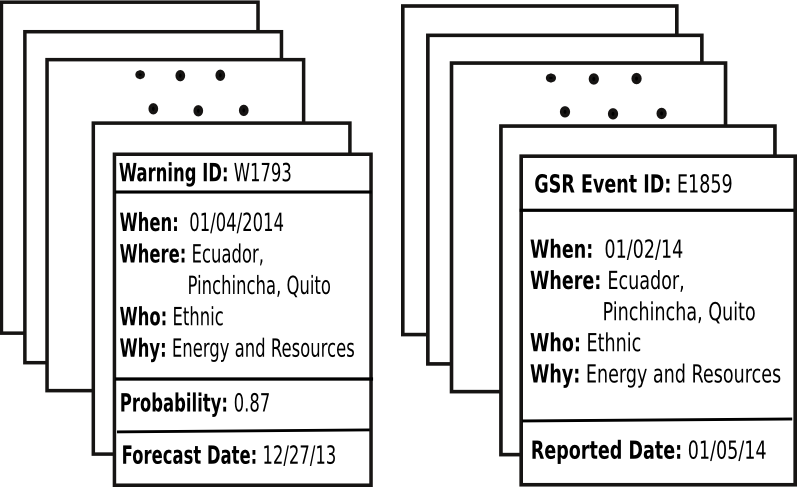
\includegraphics[width=0.5\textwidth]{alertstructure}
    \caption{Warnings and GSR events. \narenc{Remove probability from the left picture.}}
    \label{fig:alertstructure}
\end{figure}

Our goal is to identify calls for protests, strikes, or civil disobedience movements from news, blogs, Tweets, and Facebook
pages, with a view toward predicting the {\bf when} (date of the event) and {\bf where}, i.e.,
event location, upto a city level resolution, e.g., 
the city of {\it Tegucigalpa} in the state of {\it Francisco Morazan} in the country of {\it Honduras}).
In addition we seek to forecast the `why' and `who' of the protest.
The {\bf why} (or event type)
captures the main objective or reason for a civil unrest event,
and is meant to come from 7 broad classes (e.g., `Employment \& Wages',
`Housing', `Energy \& Resources' etc.) each of which is further categorized into
whether the event is forecast to be violent or not.
Finally, the {\bf who} (or population)
denotes common categories of human populations
used in event coding~\cite{philschrodt}
such as
Business, Ethnic, Legal (e.g. judges or lawyers), Education (e.g. teachers or students or parents of students), Religious (e.g. clergy), Medical (e.g., doctors or nurses), Media, Labor, Refugees/Displaced, Agricultural (e.g. farmers,
or just General Population. We refer to our forecasts as alerts or warnings (see Fig.~\ref{alertstructure} (left)).
In looking at the structure of the alert, it is important to distinguish between the forecast date (when the forecast is made)
and the predicted event date (i.e., the {\bf when} of the event).

To evaluate our alerts we have access to a database of protests organized by a third party (source and reference
not provided due to double blind reviewing considerations, but will be added later). We refer to this database as the
GSR (for Gold Standard Report). Human analysts scan newspapers of record in the countries of interest and catalog
protests. The structure of a GSR event (see Fig.~\ref{fig:alertstructure} (right)) is similar to that of an alert with
the only difference being that an event record captures both the reported date (i.e., the date of newspaper publication)
and the event date (i.e., when the newspaper article reports the protest as having happened).
The GSR is available from Nov 2012 \narenc{Confirm if this date is correct.} and is used in this paper primarily to 
help evaluate the performance of our system. Anectodal evidence of GSR (as mentioned in Section~\ref{intro}) revealed
that over 75\% of the protests were organized and had clear triggering circumstances with political entrepreneurs leading the
charge to protest.

%Concomitant with the definitions in the above section, a GSR event contains
%again the where/why/when/\hskip0ex who of a protest that has actually occurred and
%a {\it reported date} (the date a newspaper reports the protest as
%having happened).
%See Fig.~\ref{fig:alertstructure} (right).
%The GSR is organized by an
%independent third party (MITRE) and the authors of this study do not
%have any participation in this activity. 

%\subsection{Lead Time vs Accuracy of Forecast Date}
%Before we explain how alerts are matched to events, it is important to
%first understand which alerts {\it can} be matched to specific events.
%Note that there are four dates in an (alert,event) combination (see Fig.~\ref{fig:timeline}):
%\begin{enumerate}
%\item The date the forecast is made ({\it forecast date})
%\item The date the event is predicted to happen ({\it predicted event date})
%\item The date the event actually happens ({\it event date})
%\item The date the event is reported in a GSR source ({\it reported date})
%\end{enumerate}

%\subsection{Lead Time vs Accuracy of Forecast Date}
%Before we explain how alerts are matched to events, it is important to
%first understand which alerts {\it can} be matched to specific events.
%Note that there are four dates in an (alert,event) combination (see Fig.~\ref{fig:timeline}):
%\begin{enumerate}
%\item The date the forecast is made ({\it forecast date})
%\item The date the event is predicted to happen ({\it predicted event date})
%\item The date the event actually happens ({\it event date})
%\item The date the event is reported in a GSR source ({\it reported date})
%\end{enumerate}

\iffalse
\subsection{Quality Score}
The Quality score is defined as $$QS = (LS + DS)*2$$ where LS and DS denote location score and date score respectively. The location score is defined based on the kilometre distance between the predicted location and actual location. An alert can be matched to an event, if and only if it is within a 300km radius of the event location. The location score for an alert $Y$ with respect to an event $X$ is defined as $$LS=1 - min(dist(X,Y), 300) / 300 $$
The date score is defined similarly as $$DS = 1 - min( (X-Y), MAXINTERVAL)/MAXINTERVAL$$ where MAXINTERVAL  can be anything. For our experiments, a MAXINTERVAL of 7 days is used. Again a matching cannot occur if $DS=0$
\fi
